% proposal.tex
\documentclass[main.tex]{subfiles}
\begin{document}
\chapter{Machine Learning Techniques} \label{ch:ml}

The use of AM technologies to produce small batches of highly customized, complex parts, in a reduced development cycle results extremely attractive. While constructing failure envelopes can help overcome the wariness of industrial segments to design end-user parts, this resource is still not easy to implement, requiring a large number of mechanical tests and specialized equipment to properly map the failure behavior of a particular material. Additional complexity stems from what was shown in Chapter \ref{ch:oocrit}: processing the same material under related AM technologies yields completely different failure envelopes, implying that no generalizations should be made, and each material-process pairing needs to be studied on a case-by-case basis. In general, for AM parts to be adopted, engineers have to be able to confidently assess the probability of part failure under particular loading conditions, predict the expected mechanical properties of AM parts, and understand the underlying physics of the process. None of these conditions are completely met at the time of this work.

This work aims to provide the tools required to understand and predict mechanical performance of parts manufactured through FFF through the use of Machine Learning technologies (ML), based on process variables measured during a print using an FFF printer modified with sensors. Additionally, some, if not all of the procedures developed in this work could be extrapolated to other AM techniques.

\section{Objectives} \label{sec:objectives}

The set of printing conditions that lead to an optimal part in terms of mechanical properties aren't still fully comprehended. However, if there existed an FFF machine with in-line sensors that allowed monitoring a variety of process-variables, as well as data generated from mechanical tests and ancillary experiments, this would constitute an interesting case for development of a Machine Learning (ML) system. These excel in cases where the inputs and outcomes of a particular phenomena or task are known, but connecting the two through an explicit set of rules or relationships can result extremely complex and time consuming \cite{Chollet2018}. In this manner, ML models are \emph{trained}, as opposed to explicitly programmed, as illustrated in Figure \ref{fig:MLvsP}, where the differences between ML and traditional programming philosophies are compared. 

\begin{figure}[!htbp]
	\center
	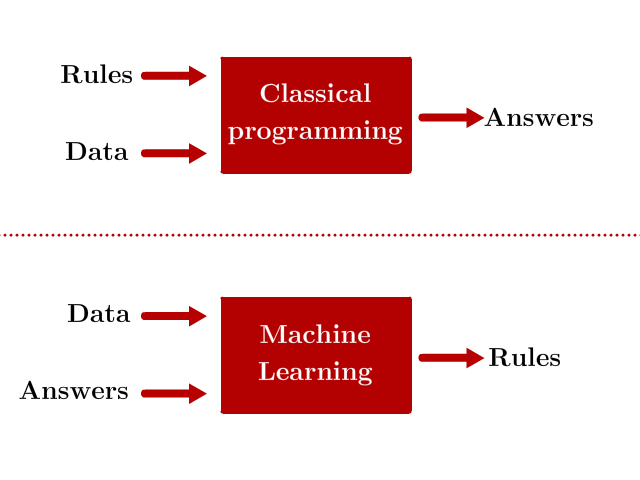
\includegraphics[height=6cm]{ML}
	\caption{Differences between traditional programming and machine learning. \cite{Chollet2018}} \label{fig:MLvsP}
\end{figure}

The potential to apply ML solutions in the field of AM has been noted by several authors \cite{Razvi2019,Meng2020}. Example cases include design-recommendation systems, topology optimization solutions, tolerancing and manufacturability assessment, and material classification and selection \cite{Razvi2019}. The specific algorithm applied for each case varied wildly depending on the nature of the task, but in general, Support Vector Machines (SVM) and Neural Networks (NN) appear to be the most prevalent solutions.

Given the factors outlined this far, the fundamental goal of this research is to predict FFF part mechanical performance by finding relations between processing conditions and strength through the use of sensors and machine learning. The success of this project would allow design engineers to confidently assess if a part manufactured through FFF will meet the mechanical requirements imposed by its intended application. This work proposes developing and using a modified printer with force and print speed sensors, as well as mechanical testing and $\mu$CT scans to generate data that can be used to train a predictive tool based on ML. This tool can then be used to predict final mechanical properties of the part based on the data generated during the print. This ML system would accept filament dimensions, printing temperature, filament force, filament velocity, print orientation, layer height, or any subset of these items as inputs, and produce final part porosity and/or mechanical strength in a particular load direction as outputs. These parameters were chosen based on previous work performed by Koch, Van Hulle and Rudolph \cite{Koch2017}, where the final tensile strength of FFF coupons was shown to be related to the morphology of the printed bead, which is significantly affected by processing parameters and variations in the volumetric output of the nozzle; research published by Sood \emph{et al.} \cite{Sood2012} where a NN was able to predict the compressive strength of FDM parts with an $R^2= 0.9977$ using layer thickness, raster angle, orientation, raster width, and air gap as inputs; as well as the proposed FFF melting models established by Bellini \emph{et al.} \cite{Bellini2004} and Osswald \emph{et al.} \cite{OsswaldMelting18}. The specifics of the architecture of the ML system are still under development, as it may prove useful to segment the problem into several sub-systems connected in series, in what is called a machine learning \emph{pipeline} \cite{Geron2019}. However, given the specifics of the task, one can conclude that the system will involve supervised learning applied to a regression problem, given that all the inputs to the system will consist of pre-selected attributes, and the mechanical response and/or porosity of a printed part can be treated as a target value the ML system has to be able to predict \cite{Mohammed2017, Meng2020}.

\begin{figure}[!htbp]
	\center
	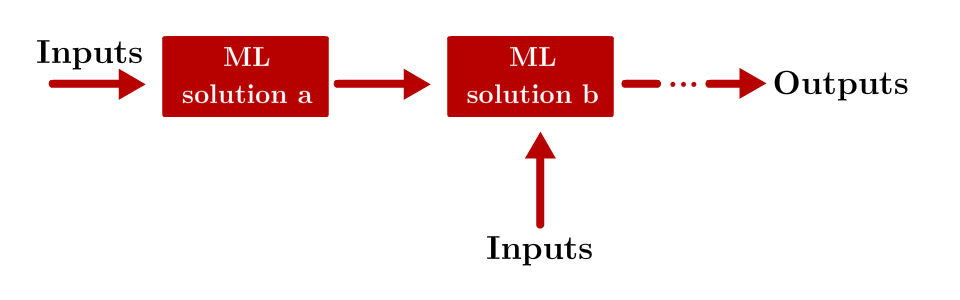
\includegraphics[height=3cm]{ML2}
	\caption{Pipeline architecture for advanced ML systems \cite{Geron2019}} \label{fig:pipeline}
\end{figure}

\begin{figure}[!htbp]
	\center
	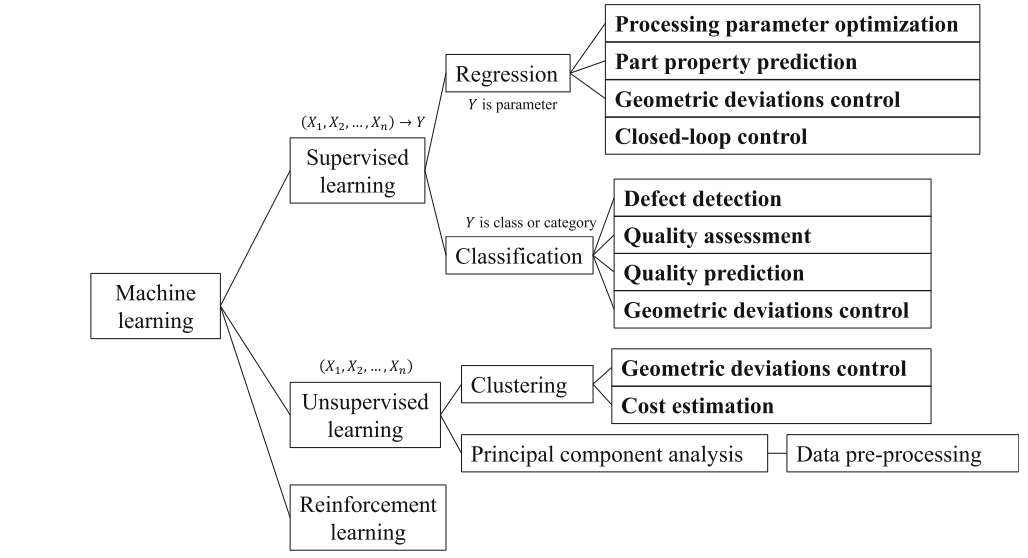
\includegraphics[height=7.5cm]{SL}
	\caption{Taxonomy of ML applications in AM \cite{Meng2020}} \label{fig:supL}
\end{figure}

\section{Preliminary results} \label{sec:prelim}

Machine learning systems require both input and output data for training and validation. Preliminary work for this study has been aimed at providing the means to supply the input piece of the puzzle. In this manner, a 3D Printer capable of capturing filament force and extrusion velocity mid-print was developed in collaboration with the company FusedForm (Bogot\'{a}, Colombia) based on their simplest commercially available product: the FusedForm Minilab. The printer was equipped with a customized force sensor and a thermistor built into the printhead, as well as an encoder that records the extruded filament length through time. The concentric force sensor was positioned just above the hot end in a bowden extruder architecture. These modifications permit recording and visualization of live force, speed, and temperature data during the printing process, while maintaining the original performance and functionality of the 3D printer intact. The generated data is then collected using an Arduino board connected to MATLAB for visualization, processing and logging. A schematic representation of the machine can be seen in Figure \ref{fig:shakira}, where dashed lines represent the path followed by the filament, and the dotted lines represent the signal sent to the Arduino board.

\begin{figure}[!htbp]
	\center
	\includegraphics[height=7cm]{forcesetup}
	\caption{Schematic of modified FFF printer with sensors} \label{fig:shakira}
\end{figure}

An initial set of experiments, designed to capture trends in filament force and velocity during a controlled print was designed. Two materials were chosen: a customized ABS filament, extruded in-house, and a commercially available PLA filament, each with a diameter of 1.75 mm. The ABS filament was produced using the SABIC Cycolac™ MG94 material. This is an ABS resin traditionally used for injection molding thin walled parts, as well as FFF filament. With a reported Melt Flow Index of 11.7 g/10 min, it is an ideal resin for both the FFF and extrusion processes \cite{sabic2016}. The extrusion setup consisted of a single screw extruder (Extrudex EDN 45X30D, Germany) with 45 mm screw diameter and L/D ratio of 30D. The hot melt was extruded at 205 ºC through a circular die with a 4.2 mm diameter. It was then guided through a pre-skinner into a vacuum-assisted, heated water bath (Conair, USA) to cool the extrudate whilst minimizing void formation. The solidified filament then passes through a 3-axis laser micrometer (LaserLinc, USA) and a belt puller (Conair, USA) in a control loop that allows adjustment of the pull speed to keep the extrudate within specification. The desired filament dimensions were a diameter of 1.75 mm with a tolerance of ± 0.02 mm. The PLA filament used was the commercially available "Natural PLA PRO" filament sold by Matterhackers \cite{MH2020}, chosen to minimize the effect of colorants/additives to the composition of the filament. Steps were taken to ensure that all the acquired spools of material came from the same lot as to guarantee that processing conditions during the extrusion process were constant. A laser micrometer was used to extract information pertaining to filament geometry, as seen in Figure \ref{fig:FD}.

\begin{figure}[!htbp]
	\center
	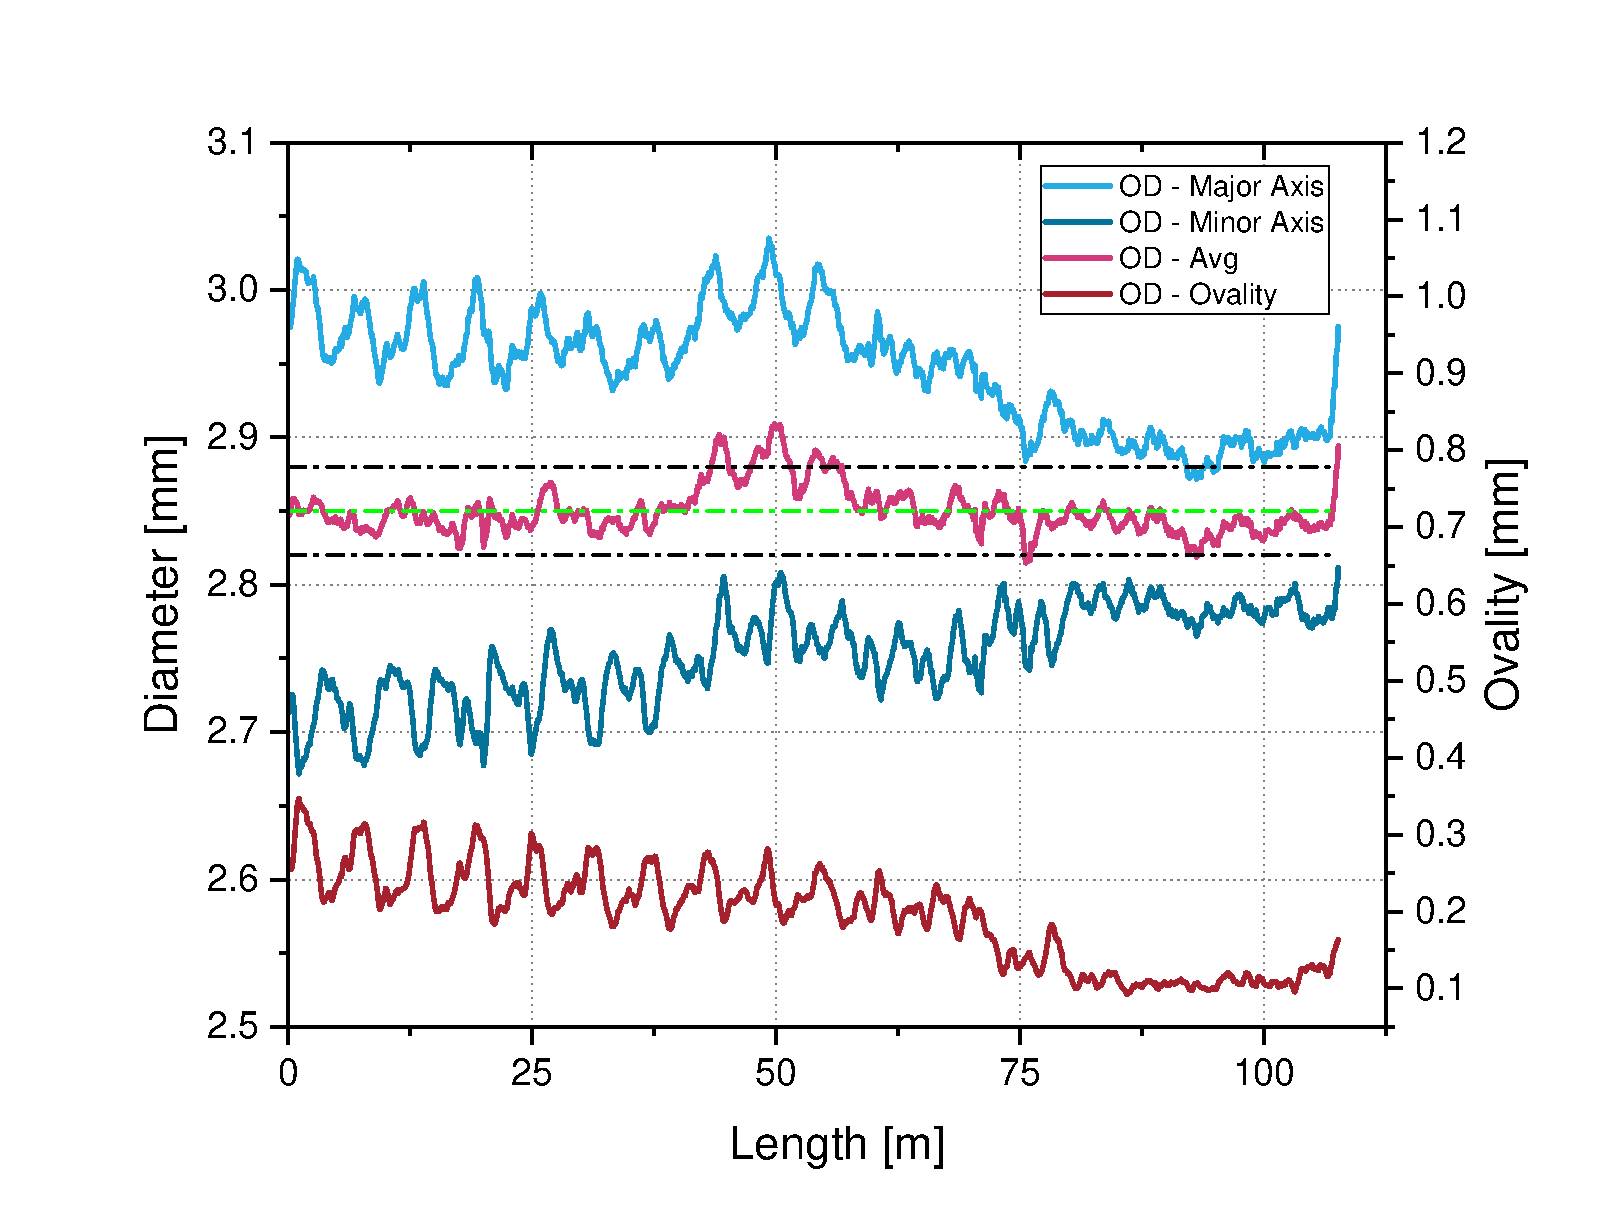
\includegraphics[width=0.7\linewidth]{FD.pdf}
	\caption{Filament geometry information, acquired through a laser micrometer } \label{fig:FD}
\end{figure}

In order to explore the effect of printing temperature and print speed upon stable printing conditions in terms of required filament force, several toolpath files were developed, where the print velocity varied was varied in increments of 5 mm/s every 15 layers, each with a thickness of 0.35 mm. To minimize the effects of varying accelerations during the test, a cylindrical geometry with a radius of 75 mm, printed in continuous helical mode was chosen as the benchmark part. This ensures that changes in filament force and velocity stem mostly from the extrusion process and not due to toolpath considerations, such as accelerations/decelerations in the X-Y plane. To verify the effect of print temperature upon the required extrusion force, each material was printed at three different temperatures: 200, 215 and 230°C for PLA, and 215, 230 and 245°C for ABS. A schematic of the print can be seen in Figure \ref{fig:cyl}.

\begin{figure}[!htbp]
	\center
	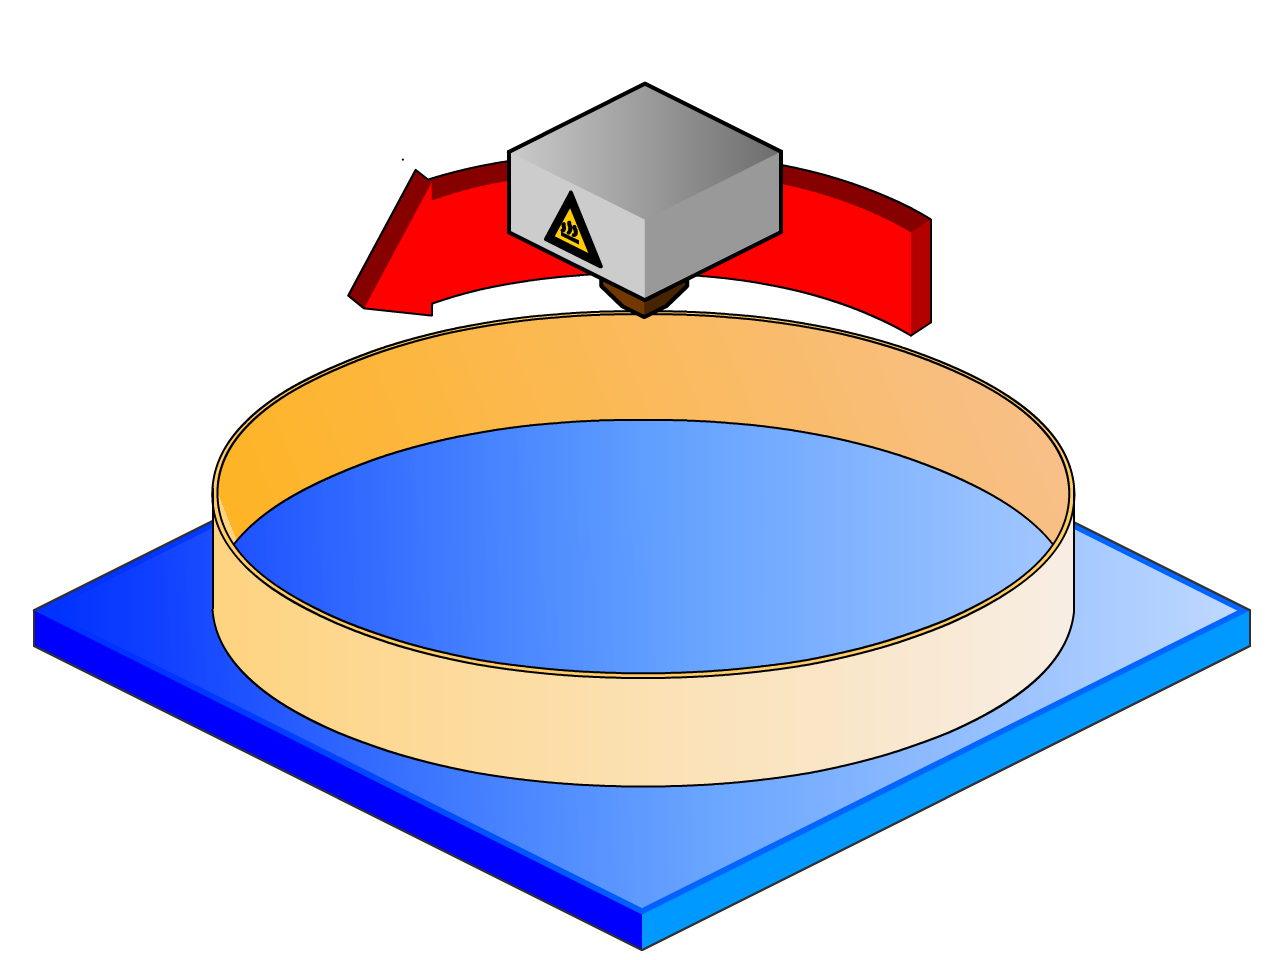
\includegraphics[width=0.6\linewidth]{cyl_shakira}
	\caption{Continuous print for force-velocity data collection} \label{fig:cyl}
\end{figure}

Preliminary results show that the physical limitation of the setup lies between 20 and 25 N of force acting upon the filament. At this level of force, slippage occurs in the drive wheel mechanism that drives the material towards the nozzle.  Increases in the hot-end temperature resulted in lower force requirements to achieve elevated printing speeds, in accordance to previous research by Go and Hart, and Go \emph{et al.} in 2017 \cite{Go2017a, Go2017}. A representative plot showing a comparison between the three print temperatures selected for ABS is shown in Figure \ref{fig:absprelim}. The data presents a significant number of noise and outliers. This is an issue that is in the process of being solved.

An interesting unexpected outcome of this set of preliminary experiments is that the trends shown in the data do not match any of the two major FFF melting models available in literature today: the Bellini model and the Osswald model \cite{Bellini2004, OsswaldMelting18}. In all permutations, the data for low speeds suggests a behavior similar to the Bellini model, but as the force-speed pairing increases, the trend is more akin to the Osswald model. Refer to Figure \ref{fig:meltmodes} for a schematic representing the observed behavior. More research is necessary to draw more definitive conclusions.

\begin{figure}[!htbp]
	\center
	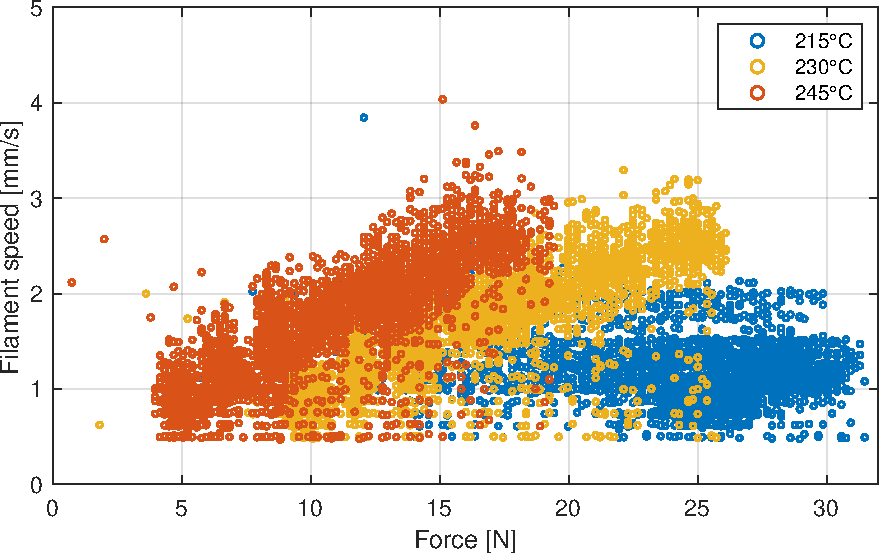
\includegraphics[width=0.8\linewidth]{ABS_prelim.pdf}
	\caption{Comparison of Force requirements for ABS at three print temperatures} \label{fig:absprelim}
\end{figure}

\begin{figure}[!htbp]
	\center
	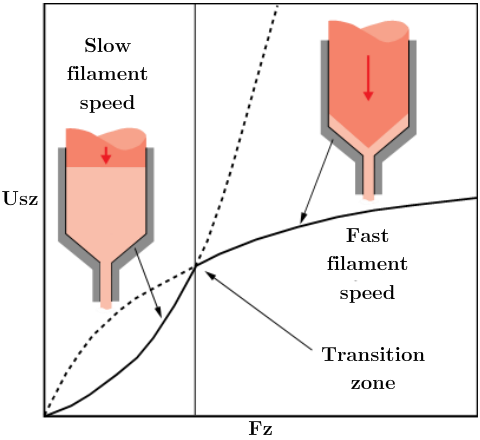
\includegraphics[width=0.7\linewidth]{meltmodes}
	\caption{Potential explanation for extrusion force-velocity trends} \label{fig:meltmodes}
\end{figure}

\section{Future work} \label{sec:fw}

The following sections describe and summarize the future research direction based on the preliminary outcomes presented in this work. 

\subsection{Data generation and preparation}\label{ssec:datag}

As seen from the preliminary experimentation, the data generated by the machine contains a noticeable number of outliers and noise. Preliminary steps would involve implementing automated data cleaning tools that ensure that the ML solution receives optimal inputs. The cylindrical print used so far would continue to act as a benchmark print given that it minimizes the impact of accelerations in the x-y plane upon the velocity-force pairings extracted from the FFF printer. Once a solution is in place, the immediate step would be the design of a mechanical coupon that consumes as little time as possible to manufacture, and that allows capturing a benchmark mechanical property through testing. An ideal initial candidate would constitute the $Y_t$ parameter used in the SSIC, given that it represents the weakest mechanical strength of FFF parts. To simplify testing and allow qualitative comparisons with the failure envelope developed by Mazzei Capote \emph{et al}. \cite{MazzeiCapote2019}, the same set of printing parameters will be used when possible. Porosity data from the prints will be extracted through $\mu$CT scans prior to testing under stress. Additional data will be supplied by measuring the filament using the laser micrometer prior to each print. Once all the experimental protocols are in place, feature selection and engineering will be required to minimize the number of inputs that are fed into the system. This includes, but is not limited to data transformation and normalization, and input aggregation. Finally, the knowledge extracted from these preliminary tests can be extrapolated for additional printing conditions and mechanical responses, constituting the entirety of the raw data that will be used with the model. At this stage, the data will be sliced into training and validation subsets, using the typical ratio of 80-20 percent if possible \cite{Geron2019}.
 
\subsection{ML system architecture, training, and validation}\label{ssec:MLA}

The following step of this work would involve using small subsets of the training data to test multiple models and algorithms in a reasonable amount of time. Performance metrics such as the Mean Square Error (MSE) or the Mean Absolute Error (MAE) would help narrow down the optimal candidate for each task \cite{Geron2019}. Depending on the outcome, the final architecture of the predictive system will be decided, including the algorithms for each segment of the machine learning pipeline if applicable. Ultimately, the final architecture of the system will be trained using the training data, and benchmarked against the validation set to check for inherent issues to the ML field, such as overfitting, and to assess the validity of the predicted outcome. The programming language of choice will be \emph{Python 3}, given its relative ease of syntax, open-source nature, as well as the availability of data science and ML libraries and resources such as \emph{NumPy, pandas, and TensorFlow}.

\begin{figure}[!htbp]
	\center
	
\includegraphics[width=0.9\linewidth]{softwareML}
	\caption{Python ML ecosystem to be used in this work} \label{fig:python}
\end{figure} 

\section{Derived Publications}

The list below represents publications derived directly from the content of this work. These are presented in chronological order.

\subsubsection{Currently published}
\begin{enumerate}
	\item \fullcite{MazzeiCapote2017}
	\item \fullcite{MazzeiCapote2018}
	\item \fullcite{MazzeiCapote2019}
	\item \fullcite{MazzeiJCompSci}
\end{enumerate}

\subsubsection{Planned publications}

The following publications are under preparation and will be submitted to the \emph{Additive Manufacturing} peer reviewed journal before the end of the year. Titles are provisional. An additional publication will be written once the final ML system is deployed.

\begin{enumerate}
	\item \fullcite{Mazzei2020}
	\item \fullcite{Osswald2020}
	\item \fullcite{Mazzei2020b}
\end{enumerate}

\pagebreak

\subsubsection{Supervised works}
During the course of this research, the author has been responsible for supervising the following works, presented in chronological order:

\begin{enumerate}
	\item \fullcite{Durris2018} % Thibaut Durris (Semester thesis)
	\item \fullcite{Bustos2020} % Max Bustos (Semester thesis)
\end{enumerate}

%______________________________________________________________________________________________
% Nomenclature introduced in this chapter:
\nomenclature[A]{ML}{Machine Learning}% 
\nomenclature[A]{SVM}{Support Vector Machines}%
\nomenclature[A]{NN}{Neural Network}%
\nomenclature[A]{MSE}{Mean Square Error}%
\nomenclature[A]{MAE}{Mean Absolute Error}%

% Symbols introduced in this chapter:
%\nomenclature[S]{$X_t$}{Tensile strength in the 1-1 direction \nomunit{$MPa$}}
\end{document}